\documentclass[11pt,letterpaper]{exam}
\usepackage{../study_session}
\usepackage{graphicx}

\pagestyle{headandfoot}
\runningheadrule
\firstpageheadrule

\firstpageheader{COMP 1805}{Study Session Practice Questions}{\today}
\runningheader{COMP 1805}{Study Session Practice Questions}{Page \thepage\ of \numpages}
\runningfooter{}{}{}

\title{COMP 1805 Discrete Structures I}
\author{Study Session Questions}

\begin{document}
\maketitle
\vspace{1em}

\begin{questions}

\section*{Proofs}

\longanswer{PROVE/DISPROVE: If $x$ and $y$ are rational numbers, then $x \cdot y$ is a rational number.}

\longanswer{Prove or disprove the converse of (a).}

\longanswer{For all integers $n > 1$, $n$ can be written as a product of primes.}

\section*{Section 1: Predicate Calculus}

\question Given $\alpha =$ True, $\beta =$ False, and $\delta =$ False, which statements are true? Select all that apply.
\begin{checkboxes}
\choice $(\alpha \lor \beta)\land \neg \delta$
\choice $(\alpha \land \beta)\lor (\neg \delta \land \alpha)$
\choice $(\beta \Rightarrow \alpha)\land (\delta \lor \alpha)$
\choice $(\alpha \land \delta)\lor (\beta \land \neg \delta)$
\choice $(\alpha \lor \neg \beta)\land (\delta \lor \beta)$
\choice none of these
\end{checkboxes}

\question Consider the statement: \emph{If it rains, then the ground is wet}. Which of the following conclusions are valid?
\begin{checkboxes}
\choice If the ground is wet, it has rained.
\choice If the ground is not wet, then it has not rained.
\choice If it does not rain, the ground will never be wet.
\choice It is not possible that the ground is dry and it is raining.
\choice none of these
\end{checkboxes}

\question Match each logical expression to its type.
\begin{matching}
\mitem{1}{$\neg((\beta \to \alpha)) \land (\beta \land \alpha)$}{A}{Contingency}
\mitem{2}{$(\alpha \to \neg \beta) \lor \neg(\alpha \lor \beta)$}{B}{Tautology}
\mitem{3}{$\neg((\neg \beta \land \neg \alpha) \land \neg(\alpha \to \beta))$}{C}{Contradiction}
\end{matching}

\question Which of the following are TRUE of a logically valid argument? Select all that apply.
\begin{checkboxes}
\choice The conclusion must be true if the premises are true.
\choice It cannot have false premises and a true conclusion.
\choice A valid argument is also sound if all premises are true.
\choice It is always a tautology.
\choice none of these
\end{checkboxes}

\question Which of the following equivalences are true for $P \Leftrightarrow Q$? Select all that apply.
\begin{checkboxes}
\choice $(P \land Q) \lor (\neg P \land Q)$
\choice $(P \lor \neg Q) \land (\neg P \lor Q)$
\choice $(P \Rightarrow Q) \land (Q \Rightarrow P)$
\choice $\neg(P \oplus Q)$
\choice False
\choice none of these
\end{checkboxes}

\question Let $P(x)$ be ``$x$ has a parking pass'' and $T(x)$ be ``$x$ has an O-Train pass''. Match each statement to its meaning.
\begin{matching}
\mitem{1}{$\forall x(P(x)\Rightarrow \neg T(x))$}{A}{Everybody who has an O-Train pass cannot have a parking pass.}
\mitem{2}{$\exists x(P(x)\Rightarrow \neg T(x))$}{B}{Someone has an O-Train pass or a parking pass.}
\mitem{3}{$\forall x(T(x)\Rightarrow \neg P(x))$}{C}{Someone has a parking pass but no O-Train pass.}
\mitem{4}{$\exists x(P(x)\lor T(x))$}{D}{Everybody who has a parking pass cannot have an O-Train pass.}
\end{matching}

\question Which of the following are logically equivalent to $\neg((P\Rightarrow Q)\land (\neg R \lor S))$? Select all that apply.
\begin{checkboxes}
\choice $(P\land \neg Q)\lor (R\land \neg S)$
\choice $(P\land \neg Q)\land (R\land \neg S)$
\choice $(P\land \neg Q)\lor (\neg(\neg R \lor S))$
\choice $(\neg P\land R)\lor (P\land \neg Q\land \neg S)$
\choice $(P\Rightarrow Q)\land (\neg R \lor S)$
\choice none of these
\end{checkboxes}

\mcquestion{Let $P(x)$ represent the statement ``$x$ is a student at CU''. Let $Q(x)$ represent the statement ``$x$ has a valid bus pass''. If $\forall x(P(x)\Rightarrow Q(x))$ is true, then which of the following must be true?}{
\choice All students at CU have a valid bus pass.
\choice Some students at CU have a valid bus pass.
\choice All people have a valid bus pass.
\choice Some people have a valid bus pass.
\choice none of these
}

\mcquestion{What is DNF of $\neg((\alpha\lor\beta)\land \neg \delta)$?}{
\choice $\neg \alpha \land \neg \beta \land \delta$
\choice $(\neg \alpha \land \neg \beta)\lor \delta$
\choice $(\neg \alpha \land \delta)\lor(\neg \beta \land \delta)$
\choice $(\neg\alpha\lor\neg \beta)\lor \delta$
}

\question Let $H(x,y)$ represent the statement ``$x$ hates $y$''. Match each statement with its meaning.
\begin{matching}
\mitem{1}{$\exists x\forall y(H(x,y))$}{A}{There is someone who hates everyone.}
\mitem{2}{$\forall x\exists y(H(x,y))$}{B}{Everybody hates someone.}
\mitem{3}{$\forall y\exists x(H(x,y))$}{C}{Everyone is hated by someone.}
\mitem{4}{$\exists y\forall x(H(x,y))$}{D}{There is someone who is hated by everyone.}
\end{matching}

\section*{Section 2: Set Theory \& Graph Theory}

\question Match each expression to its result. Let $A=\{31,12,\{23,29\},\{12,23\}\}$ and $B=\{31,\{12,23\},10,42,58\}$.
\begin{matching}
\mitem{1}{$A-B$}{A}{$\{\{31\},12,\{23,29\}\}$}
\mitem{2}{$A\cap B$}{B}{$\{10,42,58\}$}
\mitem{3}{$B-A$}{C}{$\{31,\{12,23\}\}$}
\mitem{4}{$(A\cup B)-(A\cap B)$}{D}{$\{\{31\},12,\{23,29\},31,\{12,23\}\}$}
\end{matching}

\question Which of these are equivalent to $(A\cup C)-(B\cap C)$? Select all that apply.
\begin{checkboxes}
\choice $((A-B)\cup(C-B))\cap \overline{C}$
\choice $(A\cup C)\cap(\overline{B}\cup C)$
\choice $(A\cap \overline{B})\cup C$
\choice $(A\cup C)\cap(\overline{B}\cap C)$
\choice $(A\cap C)\cup(B\cap C)$
\choice $(A\cap \overline{C})\cup(\overline{B}\cap C)$
\end{checkboxes}

\question Match each set identity to its name.
\begin{matching}
\mitem{1}{$A\cap(B\cup C)=(A\cap B)\cup(A\cap C)$}{A}{DeMorgan's Law}
\mitem{2}{$\overline{A\cup B}=\overline{A}\cap\overline{B}$}{B}{Absorption Identity}
\mitem{3}{$\overline{(\overline{A})}=A$}{C}{Distributive Law}
\mitem{4}{$A\cup(A\cap B)=A$}{D}{Double Negation}
\end{matching}

\shortanswer[1.0in]{Write the graphs in order of chromatic number (starting with the largest): $K_6$, $W_{10}$, $C_5$, $K_{3,6}$.}

\tfquestion{A tree of $n$ vertices has exactly $n-1$ edges.}


\shortanswer[0.8in]{Perform a BFS on this graph, starting from 0. Indicate the order of vertices traversed (i.e. 0 1 2 3 4 5)}


\shortanswer[0.8in]{Perform a DFS on this graph, starting from 1. Indicate the order of vertices traversed (i.e. 1 2 3 4 5 6)}

\question \textbf{} What's the adjacency list of the subgraph formed by the first 4 vertices found in a DFS, starting from (and including) 1?
\begin{choices}
\choice [[2], [5,6], [4,2], [7,2]]
\choice [[2], [1,5], [2,4], [5]]
\choice [[1], [1,2], [1,2,5], [1,2,5,4]]
\choice [[1], [1,2], [1,2,5,6], [1,2,5,6,4,7]]
\end{choices}

\question What's the adj. matrix of the subgraph formed by the first 4 vertices found in a BFS, starting from (and including) 1?
\begin{choices}
\choice $\begin{bmatrix}0&1&0&0\\1&0&1&0\\0&0&0&1\\0&0&0&0\end{bmatrix}$
\choice $\begin{bmatrix}0&1&1&1\\1&0&0&0\\1&0&0&0\\1&0&0&1\end{bmatrix}$
\choice $\begin{bmatrix}0&1&1&0\\1&0&0&1\\1&0&1&0\\0&0&0&0\end{bmatrix}$
\choice $\begin{bmatrix}0&1&1&0\\1&1&0&0\\1&0&0&1\\0&0&1&1\end{bmatrix}$
\end{choices}

\question Which of these following chemical graphs are bipartite? Select all that apply.
\begin{checkboxes}
\choice pentane\\
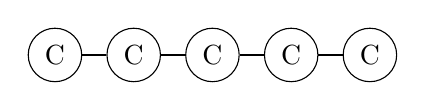
\begin{tikzpicture}[node distance=1cm, every node/.style={circle, draw, minimum size=6mm}]
  \node (1) {C};
  \node (2) [right of=1] {C};
  \node (3) [right of=2] {C};
  \node (4) [right of=3] {C};
  \node (5) [right of=4] {C};
  \draw (1) -- (2) -- (3) -- (4) -- (5);
\end{tikzpicture}

\choice cyclopentane\\
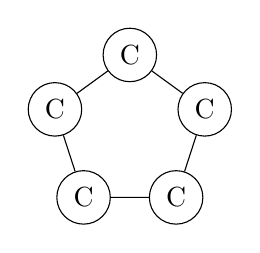
\begin{tikzpicture}[every node/.style={circle, draw, minimum size=6mm}]
  \foreach \i in {1,...,5}
    \node (\i) at ({90 + \i * 72}:1cm) {C};
  \draw (1) -- (2) -- (3) -- (4) -- (5) -- (1);
\end{tikzpicture}

\choice 2-methylbutane\\
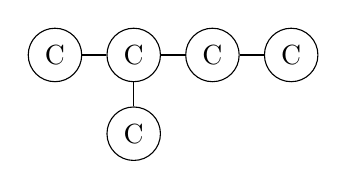
\begin{tikzpicture}[node distance=1cm, every node/.style={circle, draw, minimum size=6mm}]
  \node (1) {C};
  \node (2) [right of=1] {C};
  \node (3) [right of=2] {C};
  \node (4) [right of=3] {C};
  \node (M) [below of=2] {C};
  \draw (1) -- (2) -- (3) -- (4);
  \draw (2) -- (M);
\end{tikzpicture}

\choice 1,2,4-trimethylcyclopentane\\
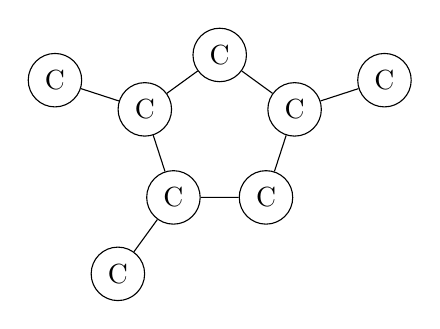
\begin{tikzpicture}[every node/.style={circle, draw, minimum size=6mm}]
  \foreach \i in {1,...,5}
    \node (\i) at ({90 + \i * 72}:1cm) {C};
  \draw (1) -- (2) -- (3) -- (4) -- (5) -- (1);

  \node (M1) at ({90 + 1 * 72}:2.2cm) {C};
  \node (M2) at ({90 + 2 * 72}:2.2cm) {C};
  \node (M4) at ({90 + 4 * 72}:2.2cm) {C};

  \draw (1) -- (M1);
  \draw (2) -- (M2);
  \draw (4) -- (M4);
\end{tikzpicture}
\end{checkboxes}

\tfquestion{If a graph contains an odd-length cycle, then it is not bipartite.}

\tfquestion{Every connected graph has a degree of at least 2.}

\longanswer{In a simple graph with 6 vertices, there exists either a connected triangle or an unconnected set of 3 vertices.}

\section*{Section 3: Everything Else}

\longanswer{Determine the maximum number of distinct primes that can divide 10 consecutive numbers.}

\question Match each expression to its series.
\begin{matching}
\mitem{1}{$\frac{n(n+1)}{4}$}{A}{$\frac14+\frac24+\frac34+\cdots+\frac{n}{4}$}
\mitem{2}{$\frac{1-(\frac13)^n}{2}$}{B}{$\frac12+\frac16+\frac1{18}+\cdots+\frac1{2\cdot 3^{n-1}}$}
\mitem{3}{$\frac{n(n+1)}{5}$}{C}{$\frac15+\frac25+\frac35+\cdots+\frac{n}{5}$}
\mitem{4}{$2\left(1-(\frac12)^2\right)$}{D}{$1+\frac12+\frac14+\cdots+\frac1{2^{n-1}}$}
\end{matching}

\longanswer{PROVE or DISPROVE: For all integers $a$ and $b$, if $a\mid b$ then $a\le b$.}

\question What can we say about $f(n)=5n\log(n)+7n+18$? Select all that apply.
\begin{checkboxes}
\choice $f(n)\in O(n\log(n))$
\choice $f(n)\in \Theta(n\log(n))$
\choice $f(n)\in \Omega(n\log(n))$
\choice $f(n)\in \Theta(n)$
\choice $f(n)\in \Omega(n)$
\end{checkboxes}

\question If $f(n)\in O(g(n))$ and $g(n)\in \Omega(h(n))$, which of the following must be true? Select all that apply.
\begin{checkboxes}
\choice $f(n)\in O(h(n))$
\choice $f(n)\in \Omega(h(n))$
\choice $f(n)\in \Omega(g(n))$
\choice $g(n)\in \Omega(f(n))$
\choice $h(n)\in O(g(n))$
\choice none of the above
\end{checkboxes}

\question Which of the following pairs $(c,k)$ can justify $2n^2+8n+20\in O(n^2)$? Select all that apply.
\begin{checkboxes}
\choice $c=2, k=2^{18}$
\choice $c=3, k=10$
\choice $c=4, k=5$
\choice $c=5, k=5$
\choice $c=2^{18}, k=0$
\choice none of the above
\end{checkboxes}

\question Which of the following expressions are true? Select all that apply.
\begin{checkboxes}
\choice $(10n-5)^2\in\Theta(n^2)$
\choice $\sqrt{n}\log(n)\in O(\log(n))$
\choice $4\log(5n^4+43n^3)\in O(\log(n))$
\choice $4n^2-n^{3/2}\in\Omega(n^3)$
\choice $30n^2-2n\in\Omega(1)$
\choice $36+\frac{1}{n^2+n}\in\Theta(1)$
\end{checkboxes}

\mcquestion{Determine the closed form of the given summation: $\sum_{i=1}^n \sum_{k=0}^{i-1} 2^k$}{
\choice $n(2^n-1)$
\choice $2^{n+1}-n-2$
\choice $\frac{2^{n+1}-2}{1-\frac12}$
\choice $2^{n-1}+n$
}

\question Indicate whether each function  is injective, surjective, both, or neither.
\begin{matching}
\mitem{1}{$f(x)=e^x$}{A}{injective}
\mitem{2}{$f(x)=x^3-3x$}{B}{surjective}
\mitem{3}{$f(x)=2x+1$}{C}{bijective}
\mitem{4}{$f(x)=\sin(x)$}{D}{neither injective nor surjective}
\end{matching}

\question Assign each relation based on its properties. Let $A=\{1,2,3\}$.
\begin{matching}
\mitem{1}{reflexive}{A}{$\{(1,1),(2,2),(3,3),(1,2)\}$}
\mitem{2}{anti-symmetric}{B}{$\{(1,2),(2,3)\}$}
\mitem{3}{transitive}{C}{$\{(1,2),(2,3),(1,3)\}$}
\mitem{4}{symmetric}{D}{$\{(1,2),(2,1)\}$}
\end{matching}

\end{questions}
\end{document}
